\documentclass{article}

\usepackage[T1,T2A]{fontenc}
\usepackage[utf8]{inputenc}
\usepackage[english,russian]{babel}

\usepackage{pdfpages}
\usepackage{multirow}

\usepackage{caption}

\usepackage{amsmath}
\usepackage[hidelinks]{hyperref}


\usepackage{graphicx}%Вставка картинок
\graphicspath{{noiseimages/}}

\usepackage{float}%"Плавающие" картинки
\usepackage{wrapfig}%Обтекание фигур (таблиц, картинок и прочего)

\makeatletter
\def\@biblabel#1{#1. }
\makeatother

\setlength{\emergencystretch}{10pt}

\begin{document}

\begin{table}[ht]
\centering
\begin{tabular}{|c|c|}
\hline
			&Потери по току	\\
\hline
Момент времени $t_1$		&0.0074\\ 
Ммомент времени $t_2$		&0.0099\\  
\hline
\end{tabular}
\caption{Противоречивые значения полученные по формуле 4.}
\end{table}

\begin{table}[ht]
\centering
\begin{tabular}{|c|c|}
\hline
			&Выход по току	\\
\hline
0		&1	\\ 
0		&1	\\  
\hline
\end{tabular}
\caption{Пустая}
\end{table}
\begin{table}[ht]
\centering
\begin{tabular}{|c|c|}
\hline
			&Выход по току	\\
\hline
0		&1	\\ 
0		&1	\\  
\hline
\end{tabular}
\caption{Пустая}
\end{table}

\begin{table}[ht]
\centering
\begin{tabular}{|c|c|}
\hline
			&Выход по току	\\
\hline
Момент времени $t_1$		&90.646	\\ 
Момент времени $t_2$		&93.594	\\  
\hline
\end{tabular}
\caption{Выход по току $\eta$.}
\end{table}

\begin{table}[ht]
\centering
\begin{tabular}{|c|c|}
\hline
			&Потери по току	\\
\hline
Момент времени $t_1$		&0.00674\\ 
Ммомент времени $t_2$		&0.00667\\  
\hline
\end{tabular}
\caption{Потери по току $\Delta \eta$.}
\end{table}

\begin{table}[ht]
\centering
\begin{tabular}{|c|c|}
\hline
Изменение выхода по току (\%)	& Изменение потерь по току (\%) \\
\hline
2.948 & -1.038\\ 
\hline
\end{tabular}
\caption{Измененние выхода по току и потерь по току.}
\end{table}




\begin{table}[ht]
\centering
\begin{tabular}{|c|c|}
\hline
			&Выход по току	\\ 
\hline
Момент времени $t_1$		&89.638	\\  
Момент времени $t_2$		&91.365	\\  
\hline
\end{tabular}
\caption{Выход по току $\eta$.}
\end{table}

\begin{table}[ht]
\centering
\begin{tabular}{|c|c|}
\hline
			&Потери по току	\\
\hline
Момент времени $t_1$		&0.00945\\
Момент времени $t_2$		&0.00928\\  
\hline
\end{tabular}
\caption{Потери по току $\Delta \eta$.}
\end{table}

\begin{table}[ht]
\centering
\begin{tabular}{|c|c|}
\hline
Изменение выхода по току (\%)	& Изменение потерь по току (\%) \\
\hline
1.727 & -1.799\\ 
\hline
\end{tabular}
\caption{Измененние выхода по току и потерь по току.}
\end{table}




\begin{table}[ht]
\centering
\begin{tabular}{|c|c|}
\hline
			&Выход по току	\\
\hline
Момент времени $t_1$	&87.048	\\  
Момент времени $t_2$	&90.037	\\  
\hline
\end{tabular}
\caption{Выход по току $\eta$.}
\end{table}
	

\begin{table}[ht]
\centering
\begin{tabular}{|c|c|}
\hline
			&Потери по току	\\
\hline
Момент времени $t_1$	&0.01188\\  
Момент времени $t_2$	&0.01173\\  
\hline
\end{tabular}
\caption{Потери по току $\Delta \eta$.}
\end{table}

\begin{table}[ht]
\centering
\begin{tabular}{|c|c|}
\hline
Изменение выхода по току (\%)	& Изменение потерь по току (\%) \\
\hline
2.948 & -1.038\\ 
\hline
\end{tabular}
\caption{Измененние выхода по току и потерь по току.}
\end{table}

Момент времени $t_1$

Момент времени $t_2$

Здесь $\mu = 10^{-5}$.

\begin{figure}[H]
\hspace*{-5cm}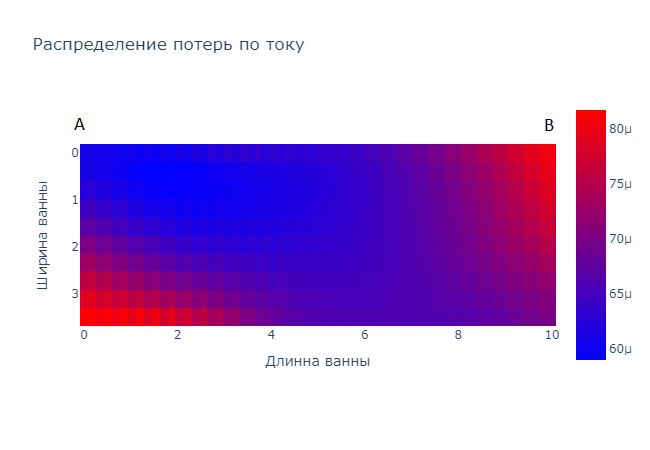
\includegraphics[width=200mm]{hloss.png}
\caption{Распределение потерь по току в ванне в стабильном состоянии.\label{fig:raspStab}}
\end{figure}

\end{document}